\hypertarget{ux6761ux4ef6ux5224ux65ad}{%
\subsection{条件判断}\label{ux6761ux4ef6ux5224ux65ad}}

\hypertarget{ux6761ux4ef6ux5224ux65ad-1}{%
\subsubsection{条件判断}\label{ux6761ux4ef6ux5224ux65ad-1}}

计算机之所以能做很多自动化的任务,因为它可以自己做条件判断。

比如,输入用户年龄,根据年龄打印不同的内容,在 Python
程序中,用\texttt{if}语句实现:

\begin{pythoncode}
age = 20
if age >= 18:
    print('your age is', age)
    print('adult')
\end{pythoncode}

根据 Python
的缩进规则,如果\texttt{if}语句判断是\texttt{True},就把缩进的两行 print
语句执行了,否则,什么也不做。

也可以给\texttt{if}添加一个\texttt{else}语句,意思是,如果\texttt{if}判断是\texttt{False},不要执行\texttt{if}的内容,去把\texttt{else}执行了:

\begin{pythoncode}
age = 3
if age >= 18:
    print('your age is', age)
    print('adult')
else:
    print('your age is', age)
    print('teenager')
\end{pythoncode}

注意不要少写了冒号\texttt{:}。

当然上面的判断是很粗略的,完全可以用\texttt{elif}做更细致的判断:

\begin{pythoncode}
age = 3
if age >= 18:
    print('adult')
elif age >= 6:
    print('teenager')
else:
    print('kid')
\end{pythoncode}

\texttt{elif}是\texttt{else\ if}的缩写,完全可以有多个\texttt{elif},所以\texttt{if}语句的完整形式就是:

\begin{pythoncode}
if <条件判断1>:
    <执行1>
elif <条件判断2>:
    <执行2>
elif <条件判断3>:
    <执行3>
else:
    <执行4>
\end{pythoncode}

\texttt{if}语句执行有个特点,它是从上往下判断,如果在某个判断上是\texttt{True},把该判断对应的语句执行后,就忽略掉剩下的\texttt{elif}和\texttt{else},所以,请测试并解释为什么下面的程序打印的是\texttt{teenager}:

\begin{pythoncode}
age = 20
if age >= 6:
    print('teenager')
elif age >= 18:
    print('adult')
else:
    print('kid')
\end{pythoncode}

\texttt{if}判断条件还可以简写,比如写:

\begin{pythoncode}
if x:
    print('True')
\end{pythoncode}

只要\texttt{x}是非零数值、非空字符串、非空 list
等,就判断为\texttt{True},否则为\texttt{False}。

\hypertarget{ux518dux8bae-input}{%
\subsubsection{再议 input}\label{ux518dux8bae-input}}

最后看一个有问题的条件判断。很多同学会用\texttt{input()}读取用户的输入,这样可以自己输入,程序运行得更有意思:

\begin{pythoncode}
birth = input('birth: ')
if birth < 2000:
    print('00前')
else:
    print('00后')
\end{pythoncode}

输入\texttt{1982},结果报错:

\begin{pythoncode}
Traceback (most recent call last):
  File "<stdin>", line 1, in <module>
TypeError: unorderable types: str() > int()
\end{pythoncode}

这是因为\texttt{input()}返回的数据类型是\texttt{str},\texttt{str}不能直接和整数比较,必须先把\texttt{str}转换成整数。Python
提供了\texttt{int()}函数来完成这件事情:

\begin{pythoncode}
s = input('birth: ')
birth = int(s)
if birth < 2000:
    print('00前')
else:
    print('00后')
\end{pythoncode}

再次运行,就可以得到正确地结果。但是,如果输入\texttt{abc}呢?又会得到一个错误信息:

\begin{pythoncode}
Traceback (most recent call last):
  File "<stdin>", line 1, in <module>
ValueError: invalid literal for int() with base 10: 'abc'
\end{pythoncode}

原来\texttt{int()}函数发现一个字符串并不是合法的数字时就会报错,程序就退出了。

如何检查并捕获程序运行期的错误呢?后面的错误和调试会讲到。

\hypertarget{ux7ec3ux4e60}{%
\subsubsection{练习}\label{ux7ec3ux4e60}}

小明身高 1.75,体重 80.5kg。请根据 BMI
公式(体重除以身高的平方)帮小明计算他的 BMI 指数,并根据 BMI 指数:

\begin{itemize}
\item
  低于 18.5:过轻
\item
  18.5-25:正常
\item
  25-28:过重
\item
  28-32:肥胖
\item
  高于 32:严重肥胖
\end{itemize}

用\texttt{if-elif}判断并打印结果:

\begin{pythoncode}
# -*- coding: utf-8 -*-

height = 1.75
weight = 80.5
\end{pythoncode}

\hypertarget{ux5c0fux7ed3}{%
\subsubsection{小结}\label{ux5c0fux7ed3}}

条件判断可以让计算机自己做选择,Python 的 if\ldots elif\ldots else
很灵活。

条件判断从上向下匹配,当满足条件时执行对应的块内语句,后续的 elif 和
else 都不再执行。

 
 \begin{figure}[htp]
	\centering
	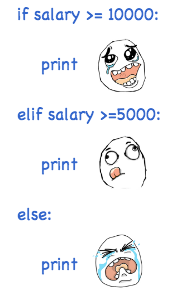
\includegraphics[width=0.6\linewidth]{fig/9240168310386880.png}
\end{figure}


\hypertarget{ux53c2ux8003ux6e90ux7801}{%
\subsubsection{参考源码}\label{ux53c2ux8003ux6e90ux7801}}

\href{https://github.com/michaelliao/learn-python3/blob/master/samples/basic/do_if.py}{do\_if.py}

